\section{\bf Introductive Remarks}

%%%%%%%%%%%%%%%%%%%%%%%%%%%%%%%%%%%%%%%%%%%%%%%%%%%%%%%%%%%%
\begin{frame}{Why Computational Chemistry?}

\onslide*<1>{

{\footnotesize
\begin{center}
	\begin{tabular}{ lrrr  }
\toprule[0.1em] 
{\bf Search query}	& {\bf Google Scholar hits}	& {\bf MathSciNet hits} & {\bf Ratio} \\
\midrule[0.08em]
\rowcolor{RedOrange}
{\sl Navier Stokes}			& 537,000		& 8,220	& 65 \\
\rowcolor{RedOrange}
{\sl Maxwell equations} 		& 194,000		& 1,892	& 102 \\
\rowcolor{YellowGreen}
{\sl Molecular dynamics} 		& 1,550,000	& 325	& 4,769 \\
\rowcolor{YellowGreen}
{\sl Density functional theory} 	& 1,200,000 	& 124 	& 9,677 \\
\rowcolor{YellowGreen}
{\sl Particle Mesh Ewald}		& 24,200 		& 1		& 24,200 \\
\rowcolor{YellowGreen}
{\sl Continuum solvation model} 	& 6,320		& 0 		&$\alert{\infty}$\\
\rowcolor{YellowGreen}
{\sl Polarizable force field}		& 3,670		& 0		&$\alert{\infty}$ \\
\bottomrule[0.1em]
	\end{tabular}
\end{center}
}

}

\onslide*<2>{

\begin{figure}
\begin{center}
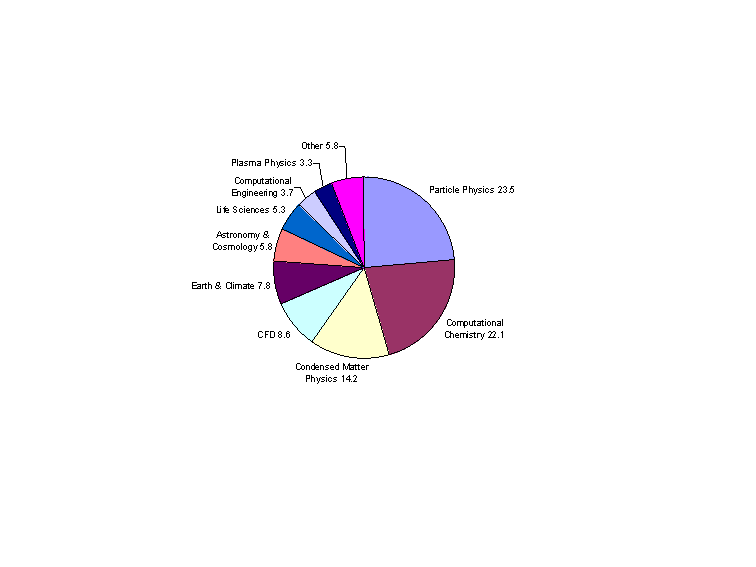
\includegraphics[scale=1]{figures/pie_chart.pdf}
\caption{Distribution of LEF's by scientific area}
\end{center}
\end{figure}

%\begin{mybox}



\begin{wideitemize}
\item {\bf Huge} usage of CPU-hours, {\bf very little} interaction with applied mathematicians
\item {\bf Great} potential for tremendous {\bf improvement}!
\end{wideitemize}


%\end{mybox}
}

\end{frame}

%%%%%%%%%%%%%%%%%%%%%%%%%%%%%%%%%%%%%%%%%%%%%%%%%%%%%%%%%%%%
\begin{frame}{Solvation Models}

\begin{figure}
\begin{center}
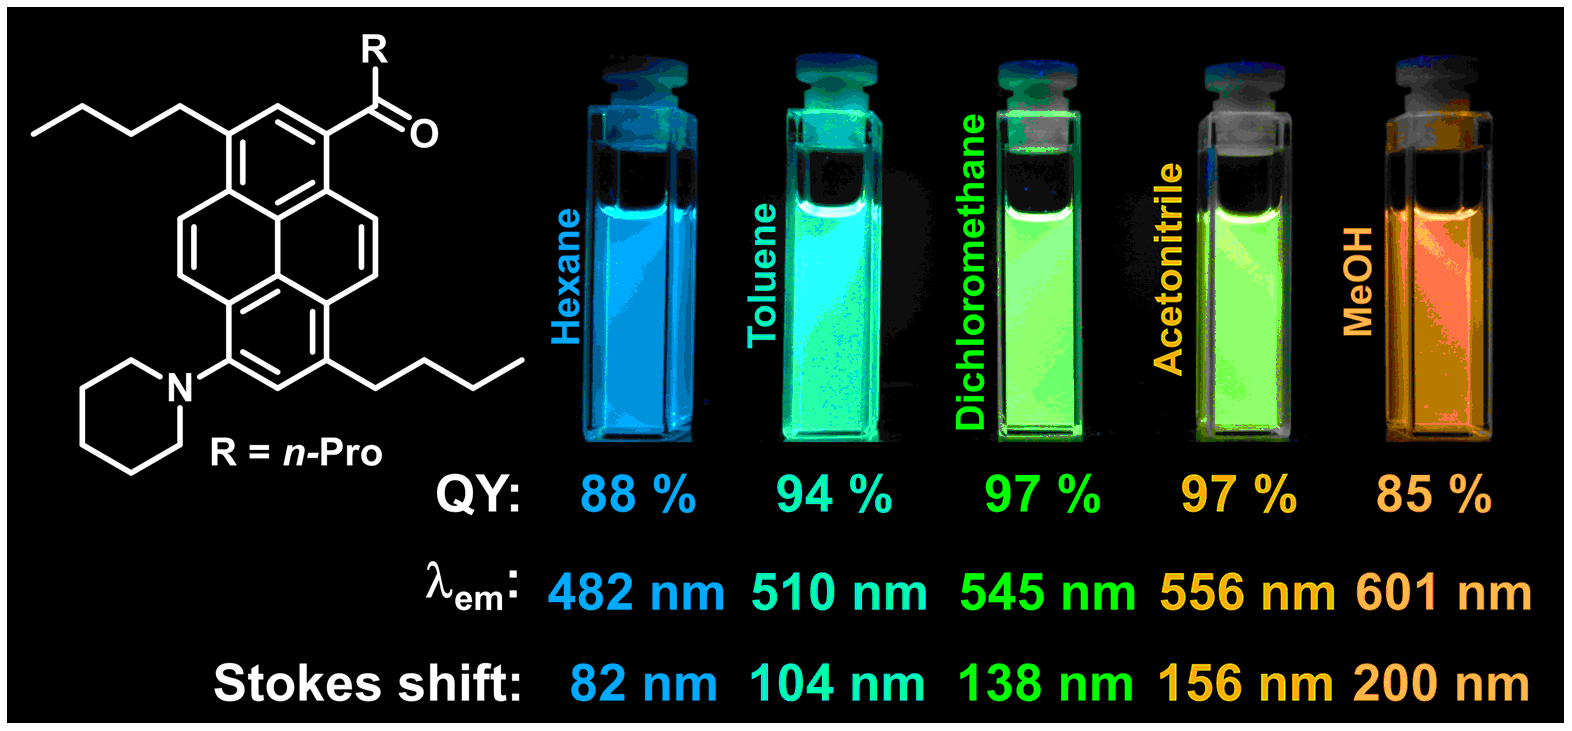
\includegraphics[trim={0cm 0cm 0cm 0cm}, width=0.78\textwidth]{figures/page11image9000.png}
%\caption{Example of Solvatochromism}
\end{center}
\end{figure}


\begin{wideitemize}
\item {\bf Several} relevant chemical phenomena take place in the {\bf liquid phase}
\item Effects of the {\bf environment} play a fundamental {\bf role}
\item {\bf \color{gray}Explicit} or {\bf implicit Solvation Models} to incorporate {\bf solvent effects} into numerical simulations.
\end{wideitemize}

\end{frame}


%%%%%%%%%%%%%%%%%%%%%%%%%%%%%%%%%%%%%%%%%%%%%%%%%%%%%%%%%%%%
\begin{frame}{Continuum Solvation Models}

%\vspace{-0.5cm}
%
%\begin{figure}
%\hfill
%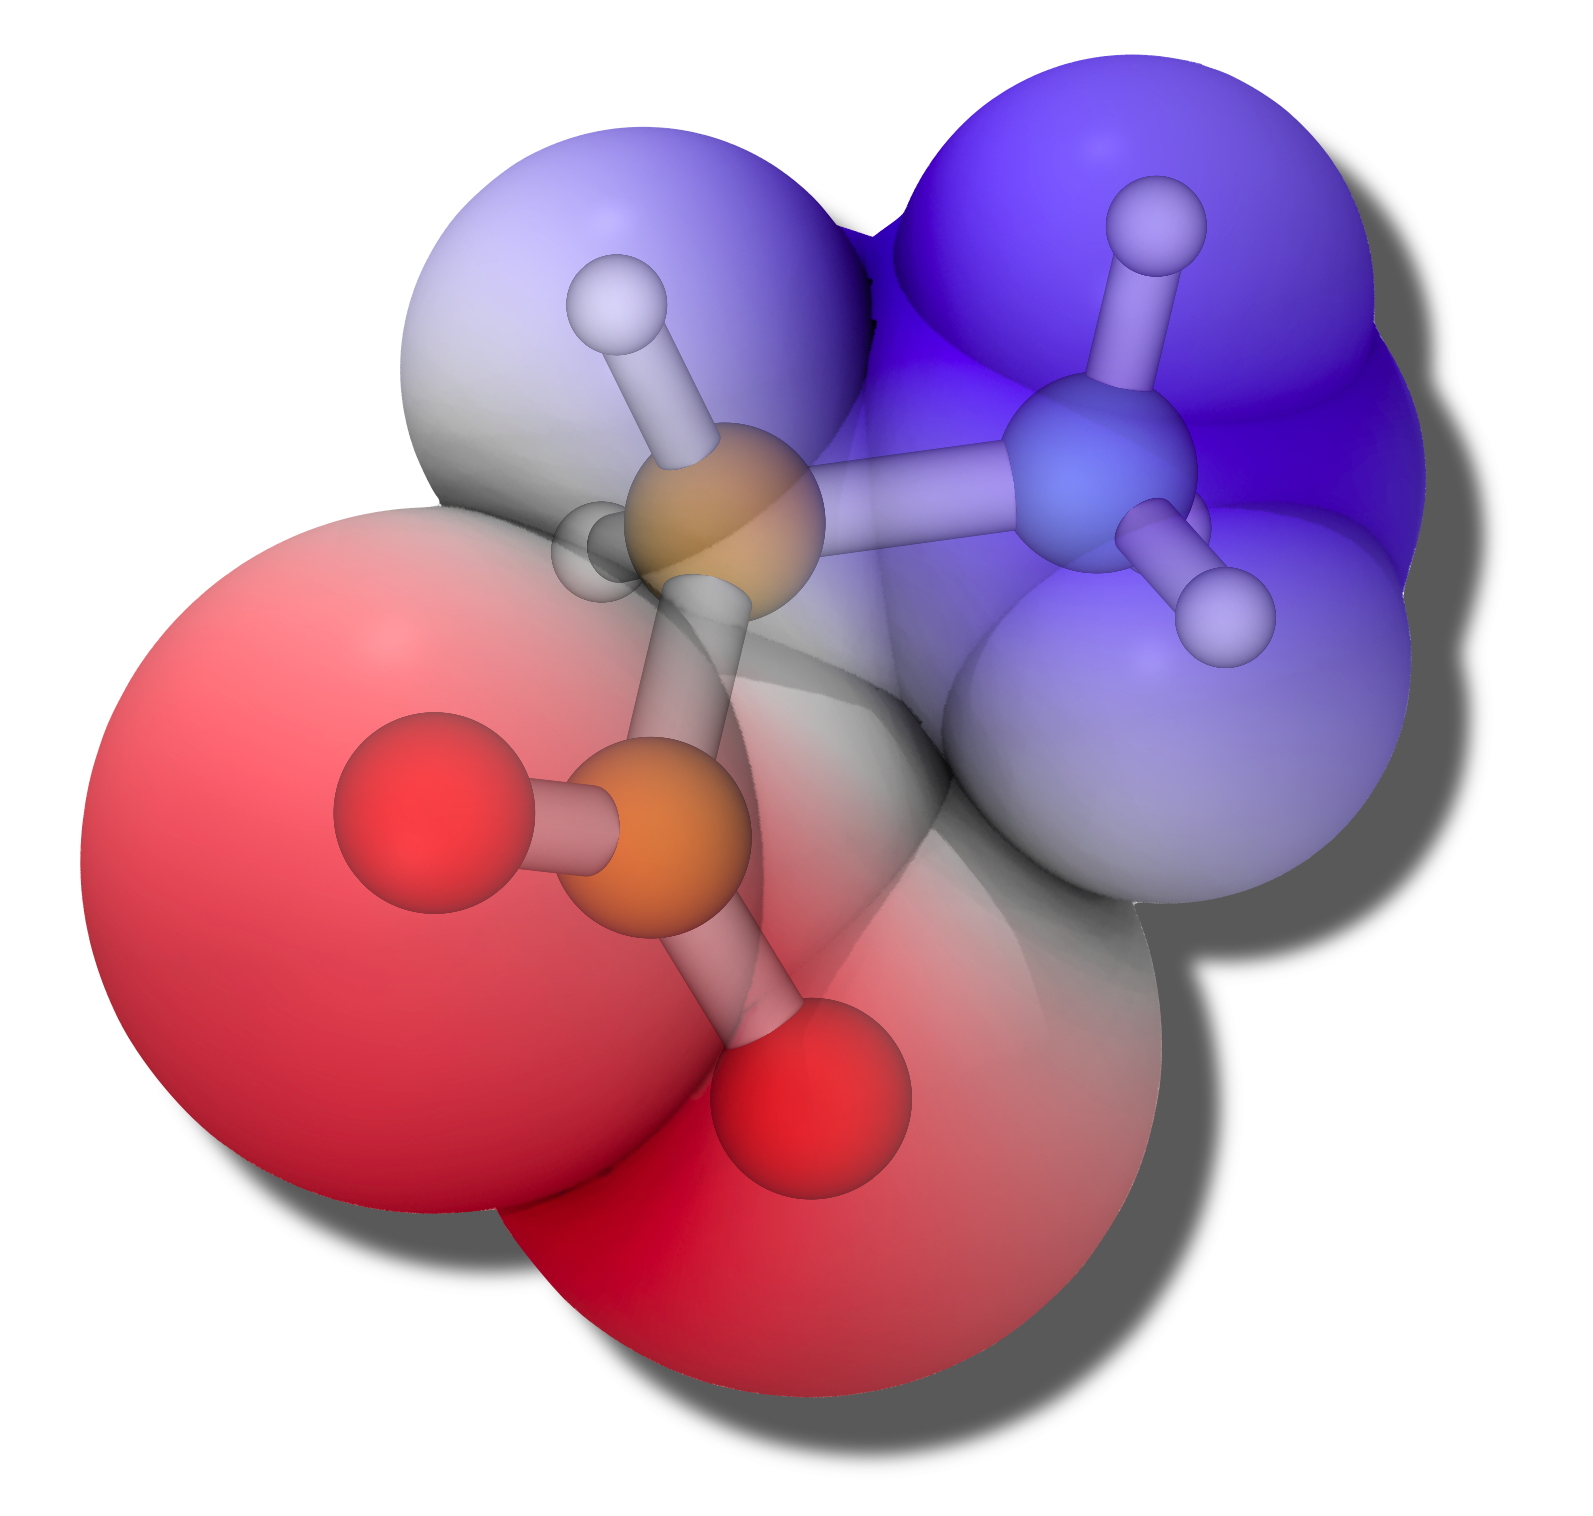
\includegraphics[trim={2cm 1cm 2cm 3cm}, width=0.25\textwidth]{figures/Cavity1.jpg}
%\end{figure}
%
%\vfill

\begin{center}
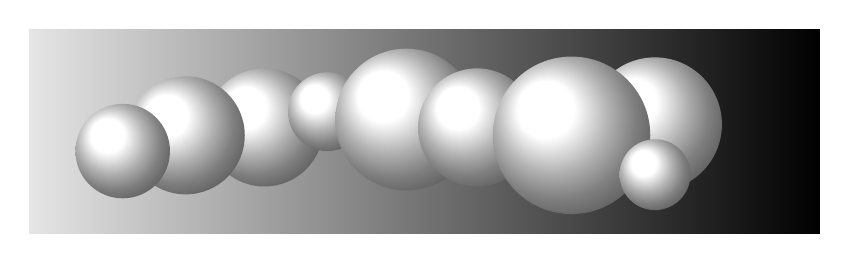
\begin{tikzpicture}[scale=0.20]
\draw [left color = black!10 , middle color = black!5, right color=black, thin, white] (-16,-6.8) rectangle (34.3,6.3);

\node[circle, shading=ball , minimum width=1.7cm ,  ball color =white ] (ball) at (23.8,0.2) {};
\node[circle,shading=ball, minimum width=1.5cm , ball color =white] (ball) at (-1,0) {};
\node[circle,shading=ball, minimum width=1cm , ball color =white] (ball) at (3,1) {};
\node[circle,shading=ball, minimum width=1.8cm , ball color =white] (ball) at (8,0.5) {};
\node[circle,shading=ball, minimum width=1.5cm , ball color =white] (ball) at (12.5,0) {};
\node[circle, shading=ball , minimum width=2cm ,  ball color =white ] (ball) at (18.5,-0.5) {};
\node[circle,shading=ball, minimum width=1.5cm , ball color =white] (ball) at (-6,-0.5) {};
\node[circle,shading=ball, minimum width=1.2cm , ball color =white] (ball) at (-10,-1.5) {};
\node[circle, shading=ball , minimum width=0.9cm ,  ball color =white ] (ball) at (23.8,-3) {};
\end{tikzpicture}
\end{center}

\begin{wideitemize}
\item {\bf Cavity} $\Omega$, bounded by a {\bf solvent excluded surface} accommodates {\bf solute}
\item Typically, $\Omega$ is a {\bf Van der Waals} cavity
\[
\Omega = \textstyle \bigcup_{\,j=1}^{\,M} \: \Omega_j \qquad ; \qquad \Omega_j = B(x_j, r_j) \qquad , \qquad r_j = \textsl{\footnotesize Van der Waals radius} \displaybump
\]
%, i.e., union of {\bf spheres} $\Omega_j = B(x_j, r_j)$, one per atom
\item Infinite {\bf continuum} replaces individual {\bf solvent} molecules
\item Solute/solvent interaction modeled as {\bf electrostatic interaction} %between the charge density of the solute and the continuum medium
\item {\bf Short-range} interactions (dispersion, repulsion, cavitation, etc.)~treated with {\bf empirical} expressions.
\end{wideitemize}

\end{frame}


\section{\bf Conductor-like Screening Model with Domain-Decomposition}
%%%%%%%%%%%%%%%%%%%%%%%%%%%%%%%%%%%%%%%%%%%%%%%%%%%%%%%%%%%%
\begin{frame}{The Conductor-like Screening Model (COSMO)}

%\vspace{-1.2cm}
%
%\begin{figure}
%\hfill
%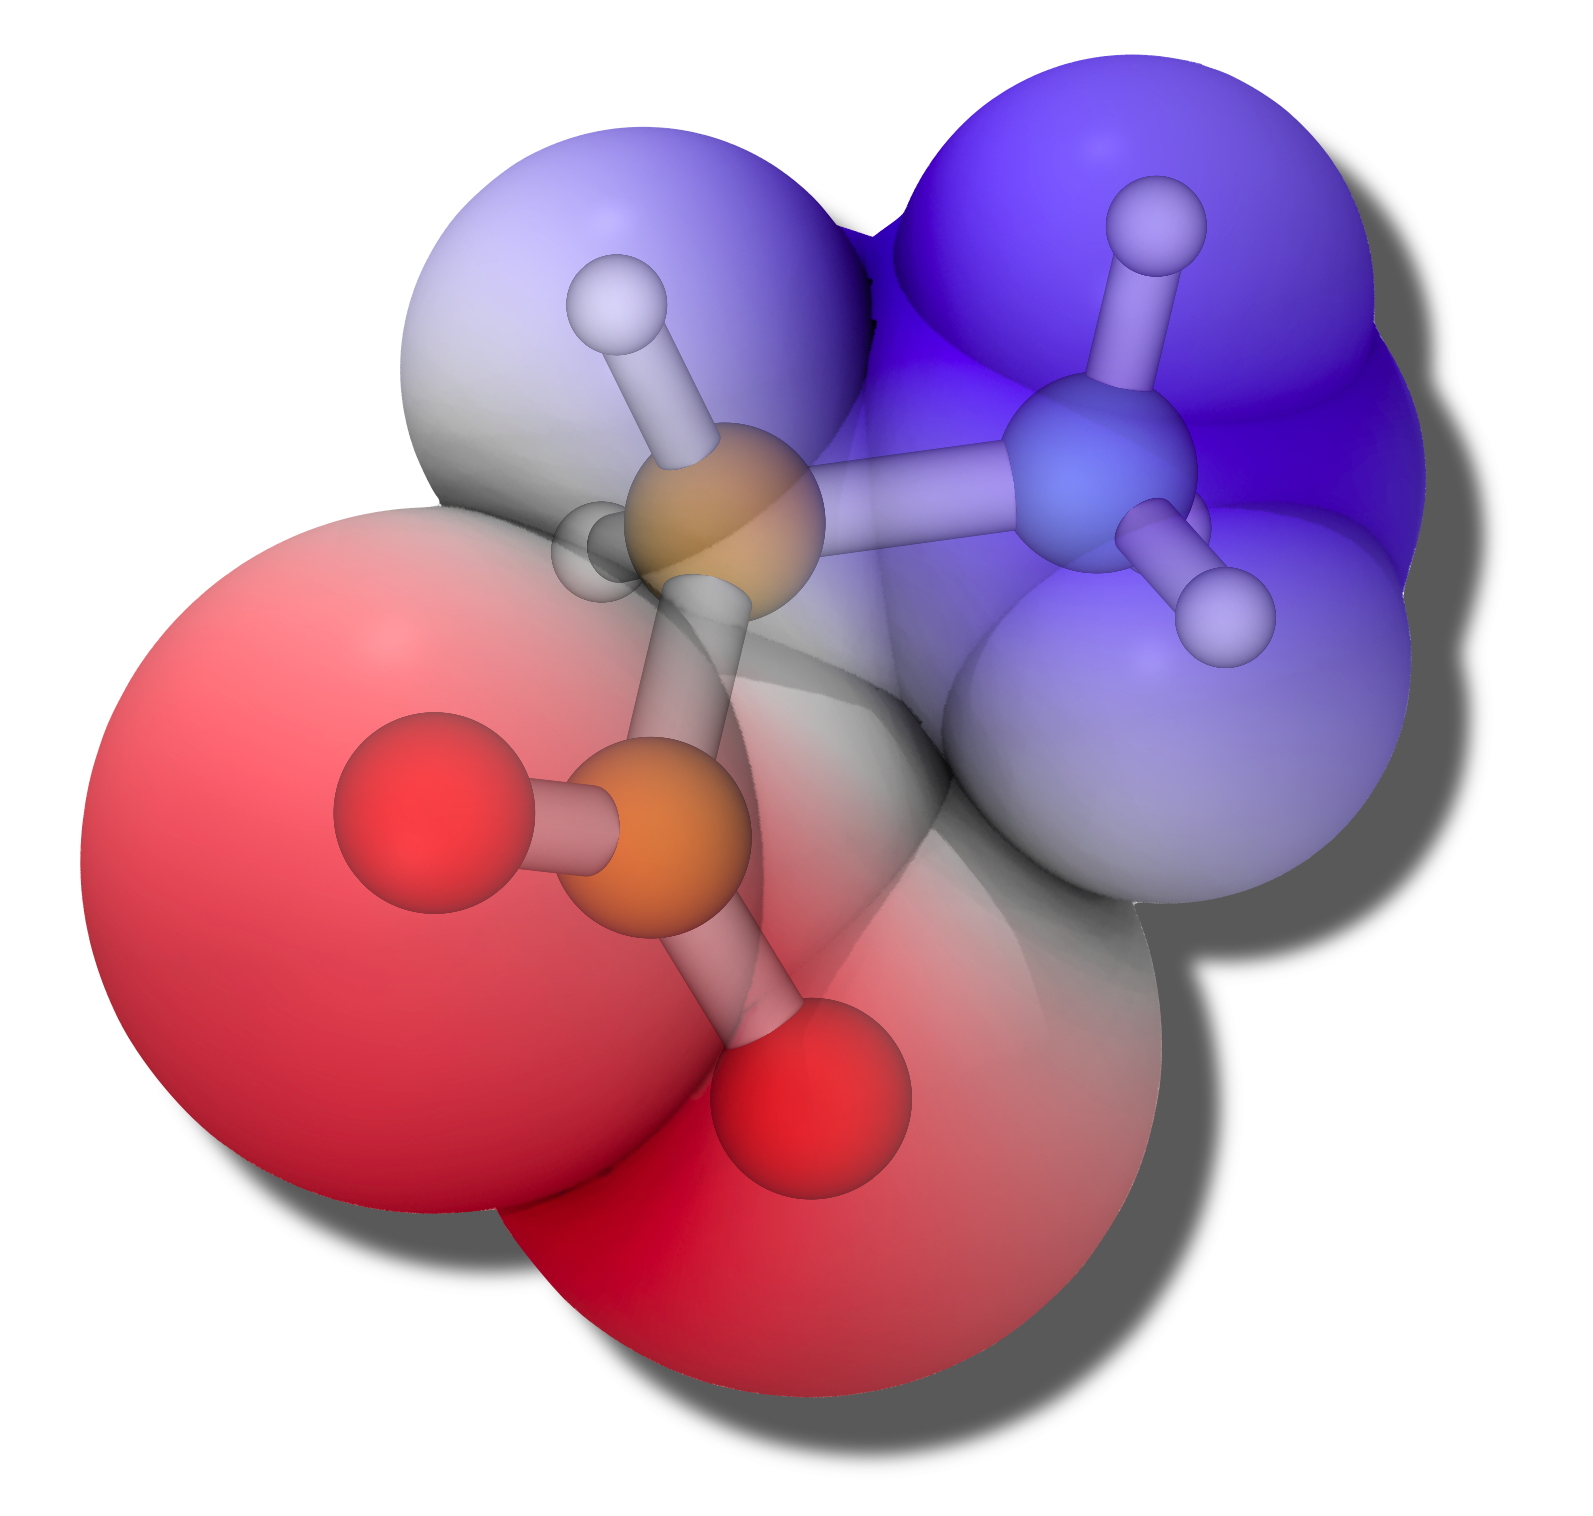
\includegraphics[trim={2cm 1cm 2cm 3cm}, width=0.25\textwidth]{figures/Cavity1.jpg}
%\end{figure}

%\vfill

\begin{wideitemize}
%\item COSMO approximates the solute/solvent {\bf interactions} as purely {\bf electrostatic forces}
\item {\bf Solvent} treated as {\bf conductor-like} medium with permittivity $\varepsilon_s \gg 1$
\item {\bf Electrostatic energy} of the solute/solvent system
\begin{align*}
E_s =\tfrac{1}{2} \;  f(\varepsilon_s)  \int_{\Omega}\varrho(x) W(x)\, dx \displaybump
\end{align*}
where $\varrho$ is the {\bf charge} density of the solute, $f(\varepsilon_s)$ is an empirical {\bf scaling}
\medskip
\item Poisson problem for {\bf reaction potential} $W$
\begin{alignat*}{3}
-\Delta \, W &= 0 &&\text{in } \Omega \displaybump \\
W &=-\Phi \qquad &&\text{on }\Gamma
\end{alignat*}
where $\Phi$ is the {\bf electric potential} generated by the solute in \emph{vacuum}.
\item Solute/solvent {\bf interaction} consists purely of {\bf electrostatic forces}.
\end{wideitemize}

\end{frame}


%%%%%%%%%%%%%%%%%%%%%%%%%%%%%%%%%%%%%%%%%%%%%%%%%%%%%%%%%%%%%
%\begin{frame}{The COSMO Implicit Solvation Model}
%
%
%
%\begin{wideitemize}
%
%\item Let $\varrho$ be the {\bf charge} density of the solute; let $W$ be the {\bf reaction potential} of the solvent
%\item The total {\bf electrostatic energy} of the solute/solvent system is given by
%\begin{align*}
%E_s =\tfrac{1}{2} \;  f(\varepsilon_s)  \int_{\Omega}\varrho(x) W(x)\, dx
%\end{align*}
%where $f(\varepsilon_s)$ is an empirical scaling factor
%\medskip
%\item The reaction potential $W$ satisfies the {\bf boundary value problem}
%\begin{alignat*}{3}
%-\Delta \, W &= 0 &&\text{in } \Omega \\
%W &=-\Phi \qquad &&\text{on }\Gamma
%\end{alignat*}
%where $\Phi$ is the {\bf electric potential} generated by the solute in vacuum
%\end{wideitemize}
%
%\end{frame}


%%%%%%%%%%%%%%%%%%%%%%%%%%%%%%%%%%%%%%%%%%%%%%%%%%%%%%%%%%%%%
%\begin{frame}{Solving the Laplace Equation}
%
%\begin{itemize}
%\item \textit{Naive Approach:} Use Finite Element methods.
%
%\begin{itemize}
%\item[--] Requires creating a 3-D mesh on the entire cavity $\Omega$.
%
%\item[--] FEM is usually applied to non-homogenous Elliptic PDEs. Would need to apply a lifting to Equation \eqref{eq:2}.
%\end{itemize}
%\medskip
%\item \textit{Convential Approach:} Recast Equation \eqref{eq:2} as an integral equation on the boundary $\Gamma$ and solve using a Boundary Element method.
%
%\begin{itemize}
%\item[+] Only need to mesh the boundary of the cavity.
%\item[--] Results in a \textit{dense}, ill-conditioned matrix. Even iterative methods become borderline unfeasible for very large systems.
%\end{itemize}
%\end{itemize}
%\end{frame}


%%%%%%%%%%%%%%%%%%%%%%%%%%%%%%%%%%%%%%%%%%%%%%%%%%%%%%%%%%%%
\begin{frame}{Domain-Decomposition COSMO (ddCOSMO)}

\begin{wideitemize}

\item Recast Poisson problem as {\bf integral} equation for {\bf surface charge} $\sigma$
\[
W(s) = \int_\Gamma \frac{\sigma(t)}{|s - t|} \, dt =:  (\mathcal{S} \, \sigma) (s)  \qquad \Rightarrow \qquad \mathcal{S} \, \sigma = -\Phi \qquad \text{on }\Gamma \displaybump
\]
\item Apply {\bf domain-decomposition} strategy to integral equation
\[
\mathcal{S}_j \, \sigma_j  - \sum_{\alert{k \:\: : \:\: \Omega_k \text{ neighbor of }\Omega_j }} \: \widetilde{\mathcal{S}}_{jk} \, \sigma_k = -\Phi_j \qquad \text{on }\Gamma_j \qquad ; \qquad  j = 1, \ldots , M \displaybump
\]
\item Interpret each local problem in a {\bf variational} setting
\[
\int_{\Gamma_j }\mathcal{S}_j \, \sigma_j \, \tau  - \sum_{k \, \in \,  N_j } \int_{\Gamma_j } \widetilde{\mathcal{S}}_{jk} \, \sigma_k \, \tau = - \int_{\Gamma_j }\Phi_j \, \tau \qquad \forall \, \tau \displaybump
\]
\item Expand $\sigma_j$ through {\bf spherical harmonics} on unit sphere $\mathbb{S}$
\[
\sigma_j(x_j + r_j y) = \tfrac{1}{r_j}  \sum_{\ell,m}\, [X_j]_\ell^m \, Y_\ell^{\,m}(y) \qquad , \qquad y \in \mathbb{S} \displaybump
\]
\item Select {\bf spherical harmonics} as {\bf test} functions $\tau$.
%\item Replace boundary value problem by {\bf coupled local} problems
%\begin{alignat*}{3}
%- \Delta \, W_i &= 0 &&\text{in } \Omega_i \\
%W_i &=g_i \qquad &&\text{on }\Gamma_i
%\end{alignat*}
%\item Employ {\bf iterative procedure} from initial guess $W^0$
%\begin{alignat*}{3}
%- \Delta \, {W_i}^{n+1} &= 0 &&\text{in } \Omega_i \\
%{W_i}^{n+1} &= - \Phi \qquad &&\text{on }\Gamma_i^\text{ext} \\
%{W_i}^{n+1} &= {W_j}^{n} \qquad &&\text{on }\Gamma_i^\text{int}
%\end{alignat*}

\end{wideitemize}

%\vspace{0.5cm}
%
%\begin{center}
%\begin{tikzpicture}[scale=0.25]
%\draw[] (0,0) circle [radius = 5];
%\draw[] (7,0.5) circle [radius = 5];
%\node at (0,0) {$\Omega_1$};
%\node at (7,0.5) {$\Omega_2$};
%\end{tikzpicture}
%\end{center}


\end{frame}

%%%%%%%%%%%%%%%%%%%%%%%%%%%%%%%%%%%%%%%%%%%%%%%%%%%%%%%%%%%%%
\begin{frame}{ddCOSMO Discretization}

\begin{center}
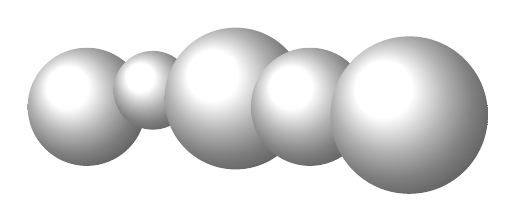
\begin{tikzpicture}[scale=0.21]
\node[circle,shading=ball, minimum width=1.5cm , ball color =white] (ball) at (-1,0) {};
\node[circle,shading=ball, minimum width=1cm , ball color =white] (ball) at (3,1) {};
\node[circle,shading=ball, minimum width=1.8cm , ball color =white] (ball) at (8,0.5) {};
\node[circle,shading=ball, minimum width=1.5cm , ball color =white] (ball) at (12.5,0) {};
\node[circle,shading=ball, minimum width=2cm , ball color =white] (ball) at (18.5,-0.5) {};
\end{tikzpicture}
\end{center}

%\begin{center}
%\begin{tikzpicture}[scale=0.23]
%%\draw [top color = olive!10 , left color = olive!10,right color = olive!10, middle color=olive , thin, white] (-13,0) rectangle (13,4.5);
%%\draw [top color = olive!10 , middle color = olive!5, bottom color=olive , thin, white] (-13,0) rectangle (13,5);
%%\draw [[top color = olive!10 , bottom color=olive , thin, white] (0,0) circle [radius = 2.5];
%\draw[fill = olive!10 , thick ] (4,1) circle [radius = 3];
%\draw[fill = olive!10 , thick] (8,0.5) circle [radius = 2];
%\draw[fill = olive!10 , thick] (12.5,0) circle [radius = 3.5];
%\draw[fill = olive!10 , thick] (17.5,-0.5) circle [radius = 2.8];
%%\draw [thick, ->] (-14,0) -- (14,0);
%%\draw [->] (0,-1) -- (0,4.5);
%%\draw [thick, ->] (-3,0) -- (-3,-2);
%\node at (0,0) {$1$};
%\node at (4,1) {$2$};
%\node at (8,0.5) {$3$};
%\node at (12.5,0) {$4$};
%\node at (17.5,-0.5) {$5$};
%%\node at (1.2,4) {$y$};
%%\node at (-4,-1) {$\boldsymbol{\nu}$};
%%\node at (-5,2.5) {$\mathbb{R}_+^{d+1}$};
%\end{tikzpicture}
%\end{center}


\begin{wideitemize}
\item Discrete operator $L$ known in {\bf closed form}, after {\bf numerical} integration
\item Operator $L$ is {\bf block-sparse}, only neighbor-to-neighbor interactions
\[ L =
{\footnotesize
\begin{pmatrix}
\times	& \times	&		& 		& \\
\times	& \times	& \times	&		& \\
		& \times	& \times	& \times	& \\
		& 		& \times	& \times 	& \times\\
		& 		&		& \times	& \times 
\end{pmatrix}
}\displaybump
\]
\item Unfortunately, operator $L$ is {\bf non symmetric}
\item Operator $L$ is {\bf well-conditioned} and {\bf diagonally dominant}
\item Employ {\bf iterative} method to solve COSMO system $L \, X = F$.
\end{wideitemize}

\end{frame}

%%%%%%%%%%%%%%%%%%%%%%%%%%%%%%%%%%%%%%%%%%%%%%%%%%%%%%%%%%%%%
\begin{frame}{How Well Are We Doing?}

\begin{wideitemize}
\item Compare to {\bf state-of-the-art}: Continuous Surface Charge (CSC) method by York and Karplus
\item CSC produces {\bf smooth energy} profiles
\item CSC is {\bf not} systematically {\bf improvable}, and {\bf poorly} conditioned.
\end{wideitemize}

\vfill

\pause

{\footnotesize
\begin{center}
\begin{table}
	\begin{tabular}{ lrrrr  }
\toprule[0.1em] 
{\bf System}	& {\bf Atoms}	& {\bf CSC} {\sl(sec)} & {\bf CSC \& FMM} {\sl(sec)} & {\bf ddCOSMO} {\sl(sec)} \\
\midrule[0.08em]
{\sl Vancomycin}	& 377	& 20  	& 43 		&  \cellcolor{YellowGreen} $<\,$1 \\
{\sl Hiv-1-GP41} 	& 530	& 86		& 57 		& \cellcolor{YellowGreen}$<\,$1 \\
{\sl l-Plectasin} 		& 567	& 96		& 77		& \cellcolor{YellowGreen}$<\,$1 \\
{\sl Glutaredoxin} 	& 1,277 	& 534 	& 182 	& \cellcolor{YellowGreen}$<\,$1 \\
{\sl UBCH5B}		& 2,360 	& 94		& 378 	& \cellcolor{YellowGreen}1 \\
{\sl Carboxylase} 	& 6,605	& 777 	& 1,482	& \cellcolor{YellowGreen}3 \\
\bottomrule[0.1em]
	\end{tabular}
		\caption{{\bf Timings} for solution of CSM/ddCOSMO equations on 2*Xeon E2560 2GHz}
		\end{table}
\end{center}
}

\end{frame}


\section{\bf Polarizable Continuum Model with Domain-Decomposition}
%%%%%%%%%%%%%%%%%%%%%%%%%%%%%%%%%%%%%%%%%%%%%%%%%%%%%%%%%%%%%
\begin{frame}{Polarizable Continuum Model (PCM)}

\begin{wideitemize}

\item {\bf Solvent} treated as a {\bf dielectric} medium with finite permittivity $\varepsilon_s$ 

\item {\bf Modified} Poisson problem for {reaction potential} $W$
\begin{alignat*}{3}
- \dive ( \varepsilon \, \nabla W ) &= 0 &&\text{in } \mathbb{R}^3 \setminus \Gamma \displaybump \\
[\![W ]\!]&=0 \qquad &&\text{on }\Gamma \\
[\![ \varepsilon \, \partial_{\bnu} W ]\!] &=(\varepsilon_s - 1 ) \, \partial_{\bnu} \Phi \qquad &&\text{on }\Gamma
\end{alignat*}
where $[\![ \cdot ]\!]$ is {\bf jump} operator, and $\varepsilon(x) = 1$ if $x \in \Omega$, and $\varepsilon(x) = \varepsilon_s$ otherwise

\item Recast as {\bf integral} equation
\[
\mathcal{R}_\varepsilon \, \mathcal{S} \, \sigma = -\mathcal{R}_\infty \, \Phi \qquad \text{on }\Gamma \displaybump
\]
where $\mathcal{R}_\varepsilon = 2\pi \,g(\varepsilon_s) \, Id - \mathcal{D}$, and $\mathcal{D}$ is the {\bf double layer} operator
\item Solve as a {\bf two-step} problem involving {COSMO}
\[
\mathcal{R}_\varepsilon \, \Phi_\varepsilon =  \mathcal{R}_\infty \, \Phi \qquad \text{on } \Gamma \qquad ; \qquad
\mathcal{S} \, \sigma =  -\Phi_\varepsilon \qquad \text{on } \Gamma \displaybump
\]

\end{wideitemize}

\end{frame}

%%%%%%%%%%%%%%%%%%%%%%%%%%%%%%%%%%%%%%%%%%%%%%%%%%%%%%%%%%%%%
\begin{frame}{Domain-Decomposion PCM (ddPCM)}

\begin{wideitemize}
\item Let $\Phi_j\: , \: \Phi_{\varepsilon,j} : \Gamma_j \to \mathbb{R}$ be the {\bf trivial extensions} of $\Phi$ and $\Phi_{\varepsilon}$ to $\Gamma_j$
\item Decompose {\bf double layer} operator as sum of {\bf local} contributions
\[
(\mathcal{D} \, \Phi_{\color{Gray}{\varepsilon}})(s) = (\mathcal{D}_j \, \Phi_{{\color{Gray}{\varepsilon,}}j})(s) + \sum_{k \, \ne \, j} \, (\widetilde{\mathcal{D}}_k \, \Phi_{{\color{Gray}{\varepsilon,}}k})(s) \qquad , \qquad s \in \Gamma_j^\text{ext} := \Gamma \cap \Gamma_j \displaybump
\]
\item {\bf Localize} integral equation through {\bf characteristic} function $U_j$ of $\Gamma_j^\text{ext}$
\[
2 \pi \, g(\varepsilon_s) \, \Phi_{\varepsilon,j} - U_j \, \mathcal{D}\, \Phi_\varepsilon = 2 \pi \, \Phi_j - U_j \mathcal{D} \,\Phi \qquad \text{on }\Gamma_j \displaybump
\]
\item Apply {\bf decomposition} to obtain final form
\[
2\pi \, g(\varepsilon_s) \, \Phi_{\varepsilon,j} - U_j \bigg( {\mathcal{D}}_j \, \Phi_{\varepsilon,j} + \sum_{\alert{k \, \ne \, j}} \, \widetilde{\mathcal{D}}_{k} \, \Phi_{\varepsilon,k}  \bigg) = \textsl{\footnotesize analogous to LHS} %\\ 2 \pi \, {\Phi_j} - U_j \bigg( {\mathcal{D}}_j \,\Phi_{j} + \sum_{k \ne j} \, \tilde{\mathcal{D}}_{k} \, \Phi_{k}  \bigg) 
\qquad \text{on }\Gamma_j  \displaybump
\]
\item Interpret local problem in a {\bf variational} setting as for COSMO. %, expand $\Phi_{\varepsilon,j}$ thorough {\bf spherical harmonics}, select spherical harmonics as {\bf test} functions.

\end{wideitemize}

\end{frame}

%%%%%%%%%%%%%%%%%%%%%%%%%%%%%%%%%%%%%%%%%%%%%%%%%%%%%%%%%%%%%
\begin{frame}{ddPCM Discretization}

\begin{center}
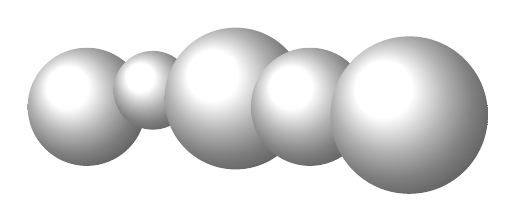
\begin{tikzpicture}[scale=0.21]
\node[circle,shading=ball, minimum width=1.5cm , ball color =white] (ball) at (-1,0) {};
\node[circle,shading=ball, minimum width=1cm , ball color =white] (ball) at (3,1) {};
\node[circle,shading=ball, minimum width=1.8cm , ball color =white] (ball) at (8,0.5) {};
\node[circle,shading=ball, minimum width=1.5cm , ball color =white] (ball) at (12.5,0) {};
\node[circle,shading=ball, minimum width=2cm , ball color =white] (ball) at (18.5,-0.5) {};
\end{tikzpicture}
\end{center}

%\begin{center}
%\begin{tikzpicture}[scale=0.23]
%%\draw [top color = olive!10 , left color = olive!10,right color = olive!10, middle color=olive , thin, white] (-13,0) rectangle (13,4.5);
%%\draw [top color = olive!10 , middle color = olive!5, bottom color=olive , thin, white] (-13,0) rectangle (13,5);
%%\draw [[top color = olive!10 , bottom color=olive , thin, white] (0,0) circle [radius = 2.5];
%\draw[fill = olive!10 , thick ] (4,1) circle [radius = 3];
%\draw[fill = olive!10 , thick] (8,0.5) circle [radius = 2];
%\draw[fill = olive!10 , thick] (12.5,0) circle [radius = 3.5];
%\draw[fill = olive!10 , thick] (17.5,-0.5) circle [radius = 2.8];
%%\draw [thick, ->] (-14,0) -- (14,0);
%%\draw [->] (0,-1) -- (0,4.5);
%%\draw [thick, ->] (-3,0) -- (-3,-2);
%\node at (0,0) {$1$};
%\node at (4,1) {$2$};
%\node at (8,0.5) {$3$};
%\node at (12.5,0) {$4$};
%\node at (17.5,-0.5) {$5$};
%%\node at (1.2,4) {$y$};
%%\node at (-4,-1) {$\boldsymbol{\nu}$};
%%\node at (-5,2.5) {$\mathbb{R}_+^{d+1}$};
%\end{tikzpicture}
%\end{center}


\begin{wideitemize}
\item Discrete operator $A_\varepsilon$ known in {\bf closed form}, after {\bf numerical} integration
\item Operator $A_\varepsilon$ is {\bf dense}, includes {\bf long-range} interactions
\[ A_\varepsilon =
{\footnotesize
\begin{pmatrix}
\times				& \times					& \alert{\boldsymbol{\times}}	& \alert{\boldsymbol{\times}} 	& \alert{\boldsymbol{\times}} \\
\times				& \times					& \times					& \alert{\boldsymbol{\times}} 	& \alert{\boldsymbol{\times}} \\
\alert{\boldsymbol{\times}}	& \times					& \times					& \times 					& \alert{\boldsymbol{\times}} \\
\alert{\boldsymbol{\times}}	& \alert{\boldsymbol{\times}}	& \times					& \times 					& \times \\
\alert{\boldsymbol{\times}}	& \alert{\boldsymbol{\times}}	& \alert{\boldsymbol{\times}}	& \times 					& \times 
\end{pmatrix}
}  \displaybump
\]
\item Unfortunately, operator $A_\varepsilon$ is {\bf non symmetric}
\item
%\item Operator $L$ is {\bf well-conditioned} and {\bf diagonally dominant}
%\item Employ {\bf iterative} method to solve COSMO system $L \, X = F$.
\end{wideitemize}


\end{frame}


%%%%%%%%%%%%%%%%%%%%%%%%%%%%%%%%%%%%%%%%%%%%%%%%%%%%%%%%%%%%%
\begin{frame}{ddPCM Forces}

\begin{wideitemize}
\item Individual {\bf domain contributions} to solvation energy
\[
E_s = \tfrac{1}{2} \, f(\varepsilon_s) \int_\Omega \varrho \, W =  \tfrac{1}{2} \, f(\varepsilon_s) \: {\textstyle \sum_{\, j}} \int_{\Omega_j} \varrho \, (\chi_j \, W) %= \cdots =  \tfrac{1}{2} \, f(\varepsilon_s)  \, \langle \Psi , X \rangle
%\: {\textstyle \sum_{\, j}} \,  {\textstyle \sum_{\, \ell,m}} \, [\Psi_j]_\ell^m \,  [X_j]_\ell^m
 \displaybump
\]
through a {\bf partition of unity} $\{\chi_j\}$
\item Approximation of {\bf local} potentials
\[
W_j (x) = (\widetilde{\mathcal{S}_j} \, \sigma_j)(x) = \sum_{\ell,m} \, [X_j]_\ell^m \, (\widetilde{\mathcal{S}}_{\, \mathbb{S}} \, Y_\ell^{\,m})(u)
% \underset{\ell,m}{\textstyle \sum} \: \tfrac{4 \pi }{2\ell + 1}\, |u|^\ell \, Y_\ell^m(u / |u|) \, [X_j]_\ell^m 
\qquad , \qquad x = x_j + r_j u  \displaybump
\]
\item Express energy as double {\bf scalar product}
\[
 E_s =\tfrac{1}{2} \,  f(\varepsilon_s) \, \langle   \Psi \, , X \rangle \qquad , \qquad \langle \cdot \, , \cdot \rangle :=  \sum_j \, \sum_{\ell,m} \, \cdots  \displaybump
 \]
where $\Psi$ is a vector {\bf independent} of nuclear positions
\item {\bf Force} acting on $i$-th atom
\[
\mathcal{F}_i = - \nabla E_s = - \tfrac{1}{2} \, f(\varepsilon_s)  \, \langle \Psi \, , \nabla X \rangle \qquad \textsl{\footnotesize gradient with respect to } x_i  \displaybump
\]
%$\langle \cdot \, , \cdot \rangle $ is a double scalar product, and $\Psi$

\end{wideitemize}

\end{frame}


%%%%%%%%%%%%%%%%%%%%%%%%%%%%%%%%%%%%%%%%%%%%%%%%%%%%%%%%%%%%%
\begin{frame}{How to Compute Forces?}

\onslide*<1>{

\vspace{0.3cm}

\begin{wideitemize}

\item {\bf Adjoint} problem $(A_\varepsilon \, L)' s = \Psi$ {\bf trasfers} operator to second argument
\[
\langle \Psi \, , \nabla X \rangle = \langle (A_\varepsilon \, L)' s \, , \nabla X \rangle = \langle  s \, , A_\varepsilon \, L \,\nabla X \rangle \displaybump
\]

\item {\bf Integration-by-parts} like approach through Leibniz rule
\begin{alignat*}{4}
A_\varepsilon \, \alert{G}& = A_\infty \, F  \qquad && \Rightarrow \qquad &  A_\varepsilon \, \alert{\nabla G} & = \nabla A ( F -G) + A_\infty \, \nabla F \displaybump \\
L \, \alert{X} & = \alert{G} &&\Rightarrow  &L \, \alert{\nabla X} & = \alert{\nabla G} - \nabla L \,  X
\end{alignat*}
\item Put it {\bf all together}, recalling intermediate solves $L' \, y= \Psi$ and $A_\varepsilon' \, s = y$
\begin{multline*}
\langle  s \, , A_\varepsilon \, L \,\alert{\nabla X} \rangle = \langle  s \, , A_\varepsilon \, \alert{\nabla G} \rangle -\langle  s \, ,A_\varepsilon \,  \nabla L \,  X  \rangle = \\
\phantom{A_\varepsilon'}= \langle  s \, ,\nabla A ( F - G) \rangle + \langle  s \, , A_\infty \, \nabla F \rangle -\langle  s \, , A_\varepsilon \, \nabla L \,  X  \rangle \displaybump
\end{multline*}
\item Since $A_\infty' \, s = (A_\infty - A_\varepsilon)' s + y$, write as {\bf perturbation} of COSMO
\[
\langle \Psi \, , \nabla X \rangle = \langle  s \, ,\nabla A ( F - G) \rangle + \langle \underbracket{(A_\infty - A_\varepsilon)'}_{\textsl{diagonal}} s \, ,  \nabla F \rangle + \underbracket{\langle y \, , \nabla F \rangle - \langle  y \, ,  \nabla L \,  X  \rangle}_{\textsl{COSMO} \:\: , \:\: O(1)} \displaybump
\]

\end{wideitemize}

}


\onslide*<2>{

\vspace{0.3cm}

\begin{wideitemize}

\item {\bf Adjoint} problem $(A_\varepsilon \, L)' s = \Psi$ {\bf trasfers} operator to second argument
\[
\langle \Psi \, , \nabla X \rangle = \langle (A_\varepsilon \, L)' s \, , \nabla X \rangle = \langle  s \, , A_\varepsilon \, L \,\nabla X \rangle \displaybump
\]

\item {\bf Integration-by-parts} like approach through Leibniz rule
\begin{alignat*}{4}
A_\varepsilon \, \alert{G}& = A_\infty \, F  \qquad && \Rightarrow \qquad &  A_\varepsilon \, \alert{\nabla G} & = \nabla A ( F -G) + A_\infty \, \nabla F \displaybump \\
L \, \alert{X} & = \alert{G} &&\Rightarrow  &L \, \alert{\nabla X} & = \alert{\nabla G} - \nabla L \,  X
\end{alignat*}
\item Put it {\bf all together}, recalling intermediate solves $L' \, y= \Psi$ and $A_\varepsilon' \, s = y$
\begin{multline*}
\langle  s \, , A_\varepsilon \, L \,\alert{\nabla X} \rangle = \langle  s \, , A_\varepsilon \, \alert{\nabla G} \rangle -\langle  s \, ,A_\varepsilon \,  \nabla L \,  X  \rangle = \\
= \langle  s \, ,\nabla A ( F - G) \rangle + \langle A_\infty' \,  s \, ,  \nabla F \rangle -\langle A_\varepsilon' \,  s \, , \nabla L \,  X  \rangle \displaybump
\end{multline*}
\item Since $A_\infty' \, s = (A_\infty - A_\varepsilon)' s + y$, write as {\bf perturbation} of COSMO
\[
\langle \Psi \, , \nabla X \rangle = \langle  s \, ,\nabla A ( F - G) \rangle + \langle \underbracket{(A_\infty - A_\varepsilon)'}_{\textsl{diagonal}} s \, ,  \nabla F \rangle + \underbracket{\langle y \, , \nabla F \rangle - \langle  y \, ,  \nabla L \,  X  \rangle}_{\textsl{COSMO} \:\: , \:\: O(1)} \displaybump
\]

\end{wideitemize}

}

\onslide*<3>{

\vspace{0.3cm}

\begin{wideitemize}

\item {\bf Adjoint} problem $(A_\varepsilon \, L)' s = \Psi$ {\bf trasfers} operator to second argument
\[
\langle \Psi \, , \nabla X \rangle = \langle (A_\varepsilon \, L)' s \, , \nabla X \rangle = \langle  s \, , A_\varepsilon \, L \,\nabla X \rangle \displaybump
\]

\item {\bf Integration-by-parts} like approach through Leibniz rule
\begin{alignat*}{4}
A_\varepsilon \, \alert{G}& = A_\infty \, F  \qquad && \Rightarrow \qquad &  A_\varepsilon \, \alert{\nabla G} & = \nabla A ( F -G) + A_\infty \, \nabla F \displaybump \\
L \, \alert{X} & = \alert{G} &&\Rightarrow  &L \, \alert{\nabla X} & = \alert{\nabla G} - \nabla L \,  X
\end{alignat*}
\item Put it {\bf all together}, recalling intermediate solves $L' \, y= \Psi$ and $A_\varepsilon' \, s = y$
\begin{multline*}
\langle  s \, , A_\varepsilon \, L \,\alert{\nabla X} \rangle = \langle  s \, , A_\varepsilon \, \alert{\nabla G} \rangle -\langle  s \, ,A_\varepsilon \,  \nabla L \,  X  \rangle = \\
= \langle  s \, ,\nabla A ( F - G) \rangle + \langle A_\infty' \,  s \, ,  \nabla F \rangle -\langle \phantom{A_\varepsilon' } y \, , \nabla L \,  X  \rangle \displaybump
\end{multline*}
\item Since $A_\infty' \, s = (A_\infty - A_\varepsilon)' s + y$, write as {\bf perturbation} of COSMO
\[
\langle \Psi \, , \nabla X \rangle = \langle  s \, ,\nabla A ( F - G) \rangle + \langle \underbracket{(A_\infty - A_\varepsilon)'}_{\textsl{diagonal}} s \, ,  \nabla F \rangle + \underbracket{\langle y \, , \nabla F \rangle - \langle  y \, ,  \nabla L \,  X  \rangle}_{\textsl{COSMO} \:\: , \:\: O(1)} \displaybump
\]

\end{wideitemize}

}


\end{frame}


%%%%%%%%%%%%%%%%%%%%%%%%%%%%%%%%%%%%%%%%%%%%%%%%%%%%%%
\begin{frame}{Derivatives of ddPCM}

\onslide*<1>{

\begin{wideitemize}

\item Arrange computations of {\bf contraction product} as
\[
\langle s \, , \nabla A \, z \rangle = \underbracket{ s_i \sum_{\phantom{j}k\phantom{j}} \nabla_{\!i} \,A_{ik} \, z_k}_{O(M)} + \underbracket{\bigg( \sum_{j \, \ne \, i} s_j \, \nabla_{\!i} \,A_{ji}  \bigg) z_i}_{O(M)} + \underbracket{\sum_{k \, \ne \, i}\bigg(\: \sum_{j \, \ne \, i} \: s_j \, \nabla_{\!i} \,A_{ji} \, z_k \bigg) z_k}_{O(M^2)} \displaybump
\]


\item Exploit {\bf sparsity} of derivative to {\bf accelerate} computations
\begin{alignat*}{5}
\nabla_{\!i} \, A_{jj} & \quad \textsl{\footnotesize a priori nonzero} \qquad && \Leftarrow \qquad  j && \in N_i  &&\vee && j = i \\
\nabla_{\!i} \, A_{jk} & \quad \textsl{\footnotesize a priori nonzero} \qquad && \Leftarrow \qquad j && \in N_i  \quad  &&\vee  \quad && j = i \quad \vee \quad k = i \displaybump
\end{alignat*}
\[
\nabla_{\!1} \, A = {\footnotesize
\begin{pmatrix}
\times	& \times	& \times	& \times	& \times \\
\times	& \times	& \times	& \times	& \times \\
\times	&		&	&	& \\
\times	&		&	&	& \\
\times	&		&	&	&
\end{pmatrix} 
} \quad ; \quad 
\nabla_{\!2} \, A = {\footnotesize
\begin{pmatrix}
\times	& \times	& \times	& \times	& \times \\
\times	& \times	& \times	& \times	& \times \\
\times	& \times	& \times	& \times	& \times \\
		& \times	&		&		& \\
		& \times	&		&		&
\end{pmatrix}
} \quad \cdots \displaybump
\]

\pause

\item Computation of $M$ forces has {\bf quadratic} complexity.% with {\bf preconstant} depending on $L_\text{max}$, number of integration points, etc

\end{wideitemize}

}

\onslide*<2>{

\begin{wideitemize}

\item Arrange computations of {\bf contraction product} as
\[
\langle s \, , \nabla A \, z \rangle = \underbracket{ s_i \sum_{\phantom{j}k\phantom{j}} \nabla_{\!i} \,A_{ik} \, z_k}_{O(M)} + \underbracket{\bigg( \sum_{j \, \ne \, i} s_j \, \nabla_{\!i} \,A_{ji}  \bigg) z_i}_{O(M)} + \underbracket{\sum_{k \, \ne \, i}\bigg( \sum_{\alert{j \, \in \, N_i}} s_j \, \nabla_{\!i} \,A_{ji} \, z_k \bigg) z_k}_{\alert{\# \, \textsl{\footnotesize neighbors} \: \times \: O(M)}} \displaybump
\]


\item Exploit {\bf sparsity} of derivative to {\bf accelerate} computations
\begin{alignat*}{5}
\nabla_{\!i} \, A_{jj} & \quad \textsl{\footnotesize a priori nonzero} \qquad && \Leftarrow \qquad  j && \in N_i  &&\vee && j = i \\
\nabla_{\!i} \, A_{jk} & \quad \textsl{\footnotesize a priori nonzero} \qquad && \Leftarrow \qquad j && \in N_i  \quad  &&\vee  \quad && j = i \quad \vee \quad k = i \displaybump
\end{alignat*}
\[
\nabla_{\!1} \, A = {\footnotesize
\begin{pmatrix}
\times	& \times	& \times	& \times	& \times \\
\times	& \times	& \times	& \times	& \times \\
\times	&		&	&	& \\
\times	&		&	&	& \\
\times	&		&	&	&
\end{pmatrix} 
} \quad ; \quad 
\nabla_{\!2} \, A = {\footnotesize
\begin{pmatrix}
\times	& \times	& \times	& \times	& \times \\
\times	& \times	& \times	& \times	& \times \\
\times	& \times	& \times	& \times	& \times \\
		& \times	&		&		& \\
		& \times	&		&		&
\end{pmatrix}
} \quad \cdots \displaybump
\]


\item Computation of $M$ forces has {\bf quadratic} complexity.% with {\bf preconstant} depending on $L_\text{max}$, number of integration points, etc

\end{wideitemize}

}


\end{frame}